% ---------------------------------------------------------------------------
% Framework
\documentclass{paperStyle}
% !!!! Achtung: Auskommentierung des entsprechenden Seminars!!!!
\IllustrativeVisualisierung{}
% ------------------------------------------------------------------------

% for including postscript figures
% mind: package option 'draft' will replace PS figure by a filname within a frame
\ifpdf \usepackage[pdftex]{graphicx} \pdfcompresslevel=9
\else \usepackage[dvips]{graphicx} \fi


% ----------------------------------------------------------
% extra packages
% ----------------------------------------------------------
%\usepackage{cite}
\usepackage[utf8]{inputenc}
%\usepackage[hang,footnotesize]{subfigure}                %% Subfigures
\usepackage{subfigure}                %% Subfigures
\usepackage{textcomp}
\usepackage{ngerman}
\usepackage{amssymb}
\usepackage{amsmath}

\graphicspath{{figures/}}
% ----------------------------------------------------------
% some command definitions if necessary
% ----------------------------------------------------------
\makeatletter

\newcommand{\Rmnum}[1]{\textbf{\expandafter\@slowromancap\romannumeral #1@}}
\makeatother

\newcommand{\ie}{i.\,e.}
\usepackage{xcolor}
\newcommand\todo[1]{\textcolor{red}{#1}}
\setlength{\parindent}{0mm}

% ----------------------------------------------------------
% Document description
% ----------------------------------------------------------
\title{Methoden zum Finden von Feature Lines - Demarcating Curves und Photic Extremum Lines}

\author{Bastian Bernst, Jonas Englich}
\date{\today}

\begin{document}

\maketitle

\begin{abstract}
   Die Arbeit beschäftigt sich mit verschiedenen Methoden zum Finden von Feature Lines. Dabei werden insbesondere die von Kolomenkin et al. im Paper \cite{Demarcating} vorgestellten Demarcating Curves und die von Xie et al. im Paper \cite{Xie2007} vorgestellten Photic Extremum Lines betrachtet. Nach dem Einführen der Grundlagen, werden beide Konzepte zunächst erläutert und darauffolgend miteinander verglichen. Weiterhin erfolgt ein Vergleich mit anderen Methoden und das Vorzeigen der Ergebnisse.
    \\
%% Uncomment follow line and add some specific keywords for your paper
\textbf{keywords: Feature Lines, Photic Extremum Lines, Demarcating Curves}

\end{abstract}

%-------------------------------------------------------------------------
\section{Einleitung}
Linien sind ein bewährtes Mittel, um die Form und Beschaffenheit von Objekten darzustellen. Unterschiedliche Anwendungsfälle und -gebiete erfordern dabei unterschiedliche Linien zur sinnvollen Nutzung. Trotz einer großen Anzahl an Linientypen und Algorithmen gibt es noch keine optimale Allzwecklösung.
	Im Folgenden sollen die Feature Line Methoden Demarcarting Curves von Kolomenkin et al.\cite{Demarcating} und die Photic Extremum Lines von Xie et al.\cite{Xie2007} vorgestellt und bewertet werden.
\section{Grundlagen}

\subsection{Gradient}

Sei $f(x,y,z)$ ein Skalarfeld. Der Gradient $grad(f)$ ist ein Vektor, der in die Richtung der größten Änderung von f im Punkt $P(x,z,y)$ zeigt. Der Betrag des Gradienten beschreibt die Stärke dieser Änderung. Er ist definiert als der Spaltenvektor
\begin{equation}
grad(f) = \nabla f = \left(\begin{array}{c}\frac{\partial f}{\partial x} \\ \frac{\partial f}{\partial y} \\ \frac{\partial f}{\partial z}\end{array}\right)
\end{equation} 
Die Einträge des Vektors sind dabei die partiellen Ableitungen in x-,y- und z-Richtung.
\subsection{Erste und Zweite Fundamentalform}
\label{fundamental}
Gegeben sei eine durch eine offene Abbildung definierte Oberfläche $S : D \subset R^{2} \longrightarrow R^{3}$ mit den Parametern $u$ und $v$. Dann heißt die Abbildung I, die jedem Punkt $p \in S$ die Einschränkung des euklidischen Skalarproduktes auf die Tangentialebene $T_{p}S$ zuordnet \textit{Erste Fundamentalform} von S
\begin{equation}
\resizebox{.9\hsize}{!}{$
\Rmnum{1}: \mathbb{R}^{2} \rightarrow \mathbb{R}^{3}, (w_{1},w_{2}) \mapsto E(u,v)^{2} + 2F(u,v) + G(u,v)^{2}$}
\end{equation}	
Diese Form erlaubt es, Messungen innerhalb der Oberfläche vorzunehmen. Dazu gehören das Bestimmen der Länge von Kurven, der Winkel von Tangentenvektoren und des Flächeninhalts bestimmter Teilbereiche.
\\
\\
Für die in Abschnitt \ref{defpel} beschriebene Berechnung des Gradienten $\nabla f$ werden nunmehr explizit die Koeffizienten E, F und G benötigt. Diese Berechnen sich durch die partiellen Ableitungen nach den Parametern $u$ und $v$.

\begin{equation}
E(u,v) = |\frac{\partial S}{\partial u}(u,v)|^{2},
\end{equation}	
\begin{equation}
F(u,v) = \frac{\partial S}{\partial u}(u,v) \cdot \frac{\partial S}{\partial v}(u,v),
\end{equation}	
\begin{equation}
G(u,v) = |\frac{\partial S}{\partial v}(u,v)|^{2}
\end{equation}	
\\
\\	
Ist weiterhin die Fläche regulär, die erste Fundamentalform also positiv-definit, kann der Fläche ein Einheitsvektor $\vec{v}(u,v)$ zugeordnet werden. Dieser ist durch die Parameter $u$ und $v$ eines Punktes gegeben:
\begin{equation}
	\vec{v}(u,v)=\frac{X_u(u,v)\times X_v(u,v)}{|X_u(u,v)\times X_v(u,v)|}
\end{equation}
Die Koeffizienten der zweiten Fundamentalform dieses Punktes lauten dann:
\begin{equation}
	\begin{split}
	L(u,v)&= \vec{v} \cdot X_{uu}(u,v)\\
	M(u,v)&= \vec{v} \cdot X_{uv}(u,v)\\
	N(u,v)&= \vec{v} \cdot X_{vv}(u,v),
	\end{split}
\end{equation}
wobei $X_{uu}$, $X_{uv}$ und $X_{vv}$ für die zweiten partiellen Ableitungen nach den Parametern stehen. 
Weitere Darstellungsformen sind die quadratische Form:
\begin{equation}
	\Rmnum{2}: \mathbb{R}^2 \rightarrow \mathbb{R}, (w_1, w_2) \mapsto Lw_1^2+2 M w_1 w_2 + Nw_2^2,
\end{equation}
sowie die Darstellung als Matrix:
\begin{equation}
	(h_{ij}) = \begin{pmatrix}
	L & M \\
	M & N
	\end{pmatrix}
\end{equation}
Während die erste Fundamentalform $\Rmnum{1}$ Informationen über die inneren oder intrinsischen Eigenschaften einer Oberfläche liefert, können mit der zweite Fundamentalform $\Rmnum{2}$ extrinsische Eigenschaften bestimmt werden. Sie hängt von der Lage der Fläche im umgebenden Raum ab und wird zum Beispiel für die Bestimmung von Krümmungen verwendet. Für diese Arbeit istihre Bestimmung in Abschnitt \ref{implDem} zur Bestimmung des Krümmungsgradienten mit der Methode aus \cite{CurvDeriv2004} nötig.  
\subsection{Normalschnitt und Normalkrümmung}
\label{normalschnitt}
Der Normalschnitt an einem Punkt $p$ auf einer regulären Fläche im $\mathbb{R}^3$ ist die Kurve, die sich aus dem Schnitt der Oberfläche und der Ebene ergibt, die von einem Tangentialvektor $\vec{v}$ und der Normale $\vec{n}$ an diesem Punkt aufgespannt wird.\\\\Die Krümmung der ebenen Kurve, die der Normalschnitt liefert, wird auch als Normalkrümmung $\kappa$ bezeichnet:
\begin{equation}
	\kappa(v)= v^T\Rmnum{2}v
\end{equation}
Zu beachten ist hierbei, dass die Normalkrümmung an einem Punkt einer Tangentialrichtung, also der Richtung $v$ des Normalschnitts, zugeordnet wird. Die symmetrische Matrix $\Rmnum{2}$ ist die zweite Fundamentalform (\ref{fundamental}). Im Folgenden wird der Einfachheit wegen den Begriff der Krümmung verwendet. 


\section{Konzepte / Algorithmen}
Im Folgenden werden die beiden Methoden \textit{Demarcating Curves}\cite{Demarcating} und \textit{Photic Extremum Lines} \cite{Xie2007} zum Finden von Feature Lines auf 3D-Objekten vorgestellt. Es werden jeweils sowohl das Konzept und dessen Ablauf, als auch spezifische Umsetzungsdetails beschrieben.

\subsection{Demarcating Curves}\label{demcurvlabel}
Häufig reicht die reine Betrachtung eines Objektes nicht aus, um einen ausreichenden Eindruck über dessen Form und Beschaffenheit zu gewinnen. Während der Mensch mit dem Tastsinn ein weiteres Werkzeug zur Untersuchung der Oberfläche besitzt, werden in der Computergrafik Feature Lines auf dem Objekt gezeichnet. Da unterschiedliche Algorithmen auf einem Objekt zu ganz unterschiedliche Strukturen hervorheben können, existiert inzwischen eine große Menge an Methoden, die für unterschiedliche Anwendungsgebiete mal mehr, mal weniger gut geeignet sind. Kolomenkin et al. \cite{Demarcating} stellen mit den Demarcating Curves eine neue Art von Kurven vor, die vor allem auf dem Gebiet der Archäologie dabei helfen soll, Strukturen auf gefundenen Relikten sichtbar zu machen und diese zu digitalisieren.

\subsubsection{Konzept}
\label{defdem}
Betrachtet man ein Polygon-Netz einer 3D-Oberfläche (im Folgenden: Mesh) als Terrain mit Bergketten und Tälern, so verlaufen die Demarcating Curves entlang der Hänge, die Täler und Berge trennen. Sie beschreiben dabei die Orte der stärksten Beugung auf der Oberfläche, also die Orte, an denen die Ableitung der Krümmung maximal ist. Diese Punkte auf dem Mesh zu finden, ist die Aufgabe des Algorithmus.  
\\\\
Nach Rusinkiewicz \cite{CurvDeriv2004} ist die Ableitung der Krümmung durch einen $2 \times 2 \times 2$ Tensor definiert:
\begin{equation}
\label{eq:rusin}
	C = (\delta_{u1}\Rmnum{2};\delta_{u2}\Rmnum{2}) = \Big[ \Big(
	\begin{tabular}{cc}
	 a & b \\
	 b & c
	\end{tabular}\Big)
	;
	\Big(
	\begin{tabular}{cc}
	b & c \\
	c & d
	\end{tabular}
	\Big)
	\Big]
\end{equation}
$u_1$ und $u_2$ beschreiben hierbei die Hauptrichtungen. Die Ableitung der Krümmung in eine Richtung $\vec{v}$ ergibt sich aus der Multiplikation mit $C$:
$
C_{ijk} v^i v^j v^k
$.\\
\\
 Es werden nun jene Orte gesucht, an denen die Ableitung der Krümmung maximal ist. Kolomenkin et al. \cite{Demarcating} definieren dazu den Krümmungsgradienten: 
 
\textbf{Krümmungsgradient}
\emph{Der Krümmungsgradient ist die Tangentenrichtung der maximalen Abweichung der Normalkrümmung. Diese Richtung maximiert den Ausdruck: }
\begin{equation}
\label{eq:gp}
g_p= \arg\max_v C_{ijk}v^{i}v^{j}v^{k}, s.t. \Vert v\Vert = 1.
\end{equation}
Um $g_p$ zu bestimmen, kann numerisch (Sampling) oder analytisch vorgegangen werden. Kolomenkin et al. entschieden sich für eine analytische Lösung. Diese wird genauer in \ref{implDem} beschrieben. 

Aus der Definition des Krümmungsgradienten ergibt sich nun die Definition der eigentlichen Kurvenpunkte. Sie markieren die Nullstellen der Krümmung auf dem Mesh in Richtung der Krümmungsgradienten:

\textbf{Definition.} 
	\emph{\textbf{p} ist ein Punkt auf einer Demarcating Curve, wenn gilt:} \begin{equation}\label{eq:demCurve}
	\textbf{p:} \kappa(g_p) = g_p^T\Rmnum{2}g_p=0\end{equation}
 Das Vorgehen von Kolomenkin et al. bei der Ermittlung jener Punkte wird in \ref{implDem} vorgestellt. 
 
 Da alle Berechnungen direkt auf der Geometrie des Mesh stattfinden, gehören die Demarcating Curves zur Gruppe der sicht-unabhängigen Kurven. Der Verlauf der Kurven wird nicht durch den Winkel des Betrachters beeinflusst.
\begin{figure}
	\centering
	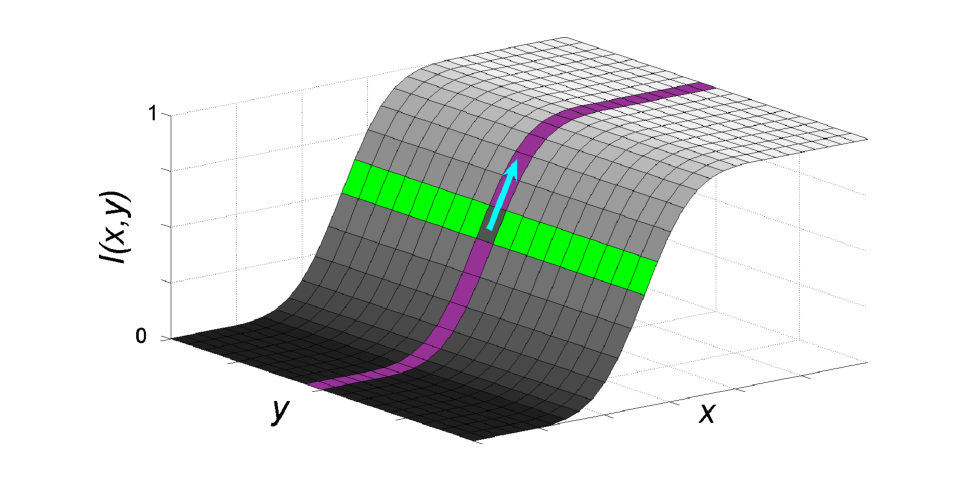
\includegraphics[width=0.9\linewidth]{demarcatingCurve.png}
	\caption{Eine weiche Stufenkante auf einem Mesh. Die Demarcating Curve (grün) verläuft orthogonal zu dem Normalschnitt (magenta) in der lokalen Richtung $g_p$ (cyan). \cite{Demarcating}}
	\label{fig:abcd}
\end{figure}
\subsubsection{Umsetzung}
\label{implDem}
 In diesem Abschnitt soll die Vorgehensweise von Kolomenkin et al. genauer erläutert werden.
 
 Wie in \ref{defdem} beschrieben, muss zunächst für jeden Vertex die Richtung des Krümmungsgradienten $g_p$ und anschließend die Krümmung  $\kappa(g_p) = g_p^T\Rmnum{2}g_p^T$ in die entsprechende Richtung bestimmt werden. Anschließend werden jene Punkte gesucht, an denen (\ref{eq:demCurve}) zutrifft, um die Kurve letztendlich zu zeichnen.
 
 \textbf{Krümmungsgradient berechnen}\\
 Um $g_p$ wie in \ref{defdem} definiert berechnen zu können, werden die zweite Fundamentalform $\Rmnum{2}$ und der Tensor $C$ für die Ableitung der Krümmung (\ref{eq:rusin}) pro Vertex bestimmt. Kolomenkin et al. verwenden dazu die Methode von S. Rusinkiewicz aus \cite{CurvDeriv2004} und implementieren sie mit der dort vorgestellten trimesh2 Bibliothek. Um anschließend $g_p$ nach Gleichung \ref{eq:gp} zu ermitteln, wählten sie einen analytischen Ansatz \cite{Demarcating}:
 
 Der Ausdruck $C_{ijk}v^iv^jv^k$ soll nach der Richtung $v$ abgeleitet und gleich Null gesetzt werden. Kolomenkin et al. bringen dazu die Gleichung \ref{eq:gp} in eine andere Form. Es sei $v=[\cos{\theta}, \sin{\theta}]$ der normierte Vektor. $a, b, c, d$ seien die Koeffizienten des Tensors aus Gleichung \ref{eq:rusin}. Danach kann Gleichung \ref{eq:gp} umgeformt werden:
 \begin{equation}
 \label{eq:gp1}
 \begin{split}
 \theta_{g_p} = \arg\max_{\theta}(a \cos^3{(\theta)} + 3b\cos^2{(\theta)}\sin{(\theta)} +\\
 + 3c\cos{(\theta)}\sin^2{(\theta)} + d\sin^3{(\theta)})
 \end{split}
 \end{equation}
 Diese Gleichung wird nach $\theta$ abgeleitet, gleich Null gesetzt und umgeformt:
 \begin{equation}
 	\label{eq:gp2}
 	\begin{split}
 	3b\cos^3(\theta) + 3(2c - a)\cos^2(\theta)\sin(\theta) + \\
 +	3(d - 2b)\cos(\theta)\sin^2(\theta) - 3c\sin^3(\theta) = 0.
 	\end{split}
 \end{equation}
 Um den Gleichung \ref{eq:gp2} weiter zu vereinfachen werden nun die höherrangigen cos Terme substituiert. Nach $cos^2(\theta) = 1 - sin^2(\theta)$ ergibt sich:
 \begin{equation}	
 \label{eq:gp3}
 \cos(\theta)=\sin(\theta)\frac{(a-3c)\sin^2(\theta)+2c-a}{(3b-d)sin^2(\theta)-b}.
 \end{equation}
 Nachdem nun der $\sin$ Term isoliert ist, können wir durch quadrieren von Gleichung \ref{eq:gp3} $\cos^2(\theta)$ endgültig entfernen:
 \begin{multline}
 \label{eq:gp4}
 	[(-3c+a)^2+(3b-d)^2\sin^6(\theta+\\
  +[2(2c-a)(-3c+a)-(3b-d)^2-2b(3b-d)]\sin^4(\theta) \\
 	+ [(2c-a)^2+2b(3b-d)+b^2]\sin^2(\theta)+-b^2=0.
 \end{multline}
 Diese Gleichung \ref{eq:gp4} ist ein Polynom dritten Grades auf $sin^2(\theta)$, somit können entweder genau eine oder drei reele Wurzeln gefunden werden, die zu zwei bzw. sechs Winkeln führen. 

 Existiert nur eine reele Wurzel, wird der Winkel des Maximums benutzt, um $g_p$ zu bestimmen. Existieren mehr als eine reele Wurzel, wird die Gleichung \ref{eq:gp1} zunächst gauss-geglättet, bevor ein globales Maximum gewählt wird. Maxima, die nahe beieinander liegen fallen so zusammen, wodurch große Maxima mehr Gewicht bekommen. 
 
 \textbf{Kurvenpunkte finden}\\
 Das Arbeiten auf einer polygonalen Oberfläche ermöglichst es zwar für jeden Vertex eine Richtung $g_p$ zu bestimmen, dabei erhält man allerdings keiner Information über die liegenden Punkte auf der Oberfläche. Da diese und verwandte Schwierigkeiten beim Umgang mit Mesh-Oberflächen verbreitete Probleme bei der Bestimmung von Kurven auf Meshes sind, existieren zahlreiche Lösungsansätze. Kolomenkin et al. orientieren sich bei ihrer Implementation an \cite{Ohtake}, \cite{DeCarlo:2007:HLF} und \cite{JuddDA07}.
 
  Um Kurvenpunkte zu erhalten die die Gleichung (\ref{eq:demCurve}) erfüllen, werden zunächst Punkte entlang der Kanten des Mesh ermittelt. Sei $p_1,p_2$ eine Meshkante. Unterscheiden sich die Vorzeichen von $\kappa(g_p1)$ und $\kappa(g_p2)$, liegt ein Kurvenpunkt auf der Kante. Die genaue Position wird durch lineare Interpolation der Krümmungen der beiden Punkte bestimmt.
 
 Bei der Suche nach den Kurvenpunkten auf den Meshkanten kommt es vor, dass die berechneten Gradientenrichtungen $g_p$ von drei Vertices eines Meshes in stark unterschiedliche Richtungen zeigen. Die Berechnung der Nullstellen der Krümmung entlang der Meshkanten liefert in diesem Fall nicht die gewünschten Punkte. Nach Gleichung \ref{eq:demCurve} in Abschnitt \ref{defdem} sollen nur die Krümmungen in eine bestimmte lokale Richtung betrachtet werden. Daher können wir zur Ermittlung der Kurvenpunkte nicht mehr einfach entlang der Kanten linear interpolieren, wenn sich die Richtungen von $g_{p_1}$, $g_{p_2}$, $g_{p_3}$ eines Dreiecks (oder Faces) $[p_1, p_2, p_3]$ stark voneinander unterscheiden. Kolomenkin et al. Lösen in Ihrem Ansatz das Problem wie folgt \cite{Demarcating}: 
 
 Unterscheiden sich die Richtungen der Gradienten dreier Vertices eines Faces stark (in \cite{Demarcating}: Winkel zwischen den Gradienten $> \pi/4$), wird dieses Face nicht weiter betrachtet. Unterscheidet sich nur eine Gradientenrichtung stark, aber die anderen beiden sind sich ähnlich, so wird der Durchschnitt der beiden ähnlichen Gradientenrichtungen bestimmt. Anschließend wird die Krümmung des dritten Vertex in diese neue Richtung bestimmt und zur Bestimmung der Kurvenpunkte verwertet. 
 
 \textbf{Achtung:} Der so berechne Gradient für den dritten Vertex liegt Möglicherweise nicht auf dessen Tangentenebene. In diesem Fall muss der Vektor rotiert werden. Dazu verweisen die Autoren auf \cite{CurvDeriv2004} und \cite{Ohtake}.
 
  Kurvenpunkte auf benachbarten Meshkanten werden schließlich durch gerade Linien verbunden, um die Kurve zu erzeugen.
\subsection{Photic Extremum Lines}
Die Beleuchtung spielt bei der menschlichen Wahrnehmung eine extrem große Rolle. Große Kontrastunterschiede sind dabei entscheidend zum Erkennen eines Objekts. Sie lassen unser Gehirn auf die Silhouette und die innere Struktur des betrachteten Objekts schließen. Die meisten Methoden, die Feature Lines auf 3D-Objekten suchen, betrachten dabei nur die Geometrie; das Verhalten unter einfallendem Licht wird ignoriert. Deshalb wurden im Jahr 2007 von der Gruppe um Xie et al. die Photic Extremum Lines (kurz: PELs) eingeführt, die sich die Beleuchtung zum Finden von Feature Lines zu Nutze macht \cite{Xie2007} .
\label{pellabel}
\subsubsection{Konzept und Ablauf}
\label{defpel}
Die Grundlage der Photic Extremum Lines stellt eine Beobachtung von A. Yuille dar, die Folgendes besagt: Untersucht man die zweite partielle Ableitung eines Schwarz/Weiss-Fotos eines Objekts in Richtung des Gradienten auf Nullstellen, so liegen diese in der Nähe der Hügel und Täler des Objekts. Diese beinhalten wiederum wichtige Informationen zur äußeren und inneren Beschaffenheit des Objekts. Xie et al. übertragen diese Beobachtung auf 3D-Oberflächen. Das Finden der Nullstellen wird also nicht auf einem Abbild des Objekts, sondern auf der beleuchteten Geometrie vollzogen.
Das grundlegende Konzept des Algorithmus lässt sich in vier Schritte unterteilen:
\begin{itemize}
\item[1.] Optional: Vorverarbeitung (Glättung der Normalen)
\item[2.] Berechnung des Gradienten für jeden beleuchteten Vektor
\item[3.] Berechnung der zweiten partiellen Ableitung in Richtung des Gradienten jedes Vektors
\item[4.] Finden der Nullstellen und Filtern der Maxima

\end{itemize}

Zur Berechnung der Nullstellen gilt die Annahme, dass die Beleuchtungsfunktion $f$ dreimal stetig differenzierbar sei (benötigt wird die dritte partielle Ableitung). \\\\
Der Gradient eines Punktes einer Oberfläche $S : D \subset R^{2} \longrightarrow R^{3}$, die mit der Beleuchtungsfunktion $f$ beleuchtet wurde, berechnet sich durch:
\begin{equation}
\nabla f = \frac{ f_{ u }G - f_{ v }F }{EG - F^{ 2 }  }S_{ u } + \frac{ f_{ v }E - f_{ u }F }{EG - F^{ 2 } } S_{ v }
	\label{eq:gradientf}
\end{equation}
$S_{ u } $ und $S_{ v }$ stehen dabei für die Tangentenvektoren des Punktes. Die jeweiligen Koeffizienten setzen sich aus den partiellen Ableitungen $f_{ u }$ und $f_{ v }$ und den Koeffizienten der zweiten Fundamentalform E,G und F des Objekts (der Oberfläche S) zusammen. Die Formeln zur Berechnung dieser Koeffizienten finden sich in Abschnitt \ref{fundamental}.

Gegeben den Gradienten $\nabla f$, kann nun die zweite Partielle Ableitung in dessen Richtung berechnet werden. Wichtig sind die Nullstellen (Extrema) der Funktion:
\begin{equation}
D_{w}||\nabla f || = 0
	\label{eq:dw}
\end{equation}
Wie in der Einleitung zu Abschnitt \ref{pellabel} bereits erwähnt, sind maximale Kontrastunterschiede (und nicht minimale) wichtig zur Darstellung der inneren und äußeren Beschaffenheit eines Objekts. Es sind deshalb nur die gefundenen Nullstellen wichtig, die ein Maxima beschreiben (in Figure \ref{fig:abcd} erkennbar). Mathematisch wird dies durch die Einschränkung
\begin{equation}
D_{w}D_{w}||\nabla f || < 0
\label{eq:dwdw}
\end{equation}
beschrieben. Es lässt sich abschließend definieren:

\textbf{Defintion.} \emph{Die PEL ist die Menge aller Punkte der Oberfläche S, die den Bedingungen (\ref{eq:dw}) und (\ref{eq:dwdw}) genügen.}\cite{Xie2007}
\\\\
Es wird deutlich, dass das Ergebnis sehr stark von der Beleuchtung des Objekts abhängt. Xie et al. schlagen deshalb sowohl eine Beleuchtungsfunktion selbst, als auch eine Positionierung der Lichter (Abschnitt \ref{belfkt}) vor.\\\\
Zu beachten ist weiterhin, dass die partiellen Ableitungen (Schritt 1,2 und 3) nicht auf kontinuierlichen Oberflächen berechnet werden, sondern die einzelnen Punkte, bzw. Dreiecke des 3D-Objekts herangezogen werden müssen. Auch die Nullstellen können nicht implizit berechnet werden, sondern müssen mittels linearer Interpolation zwischen den Ergebnissen der einzelnen Punkte gefunden werden. Die genaue Vorgehensweise wird in Abschnitt \ref{pel-impl} beschrieben, in dem zusätzlich näher auf die Vorverarbeitung der Geometrie eingegangen wird.
\begin{figure}
	\centering
		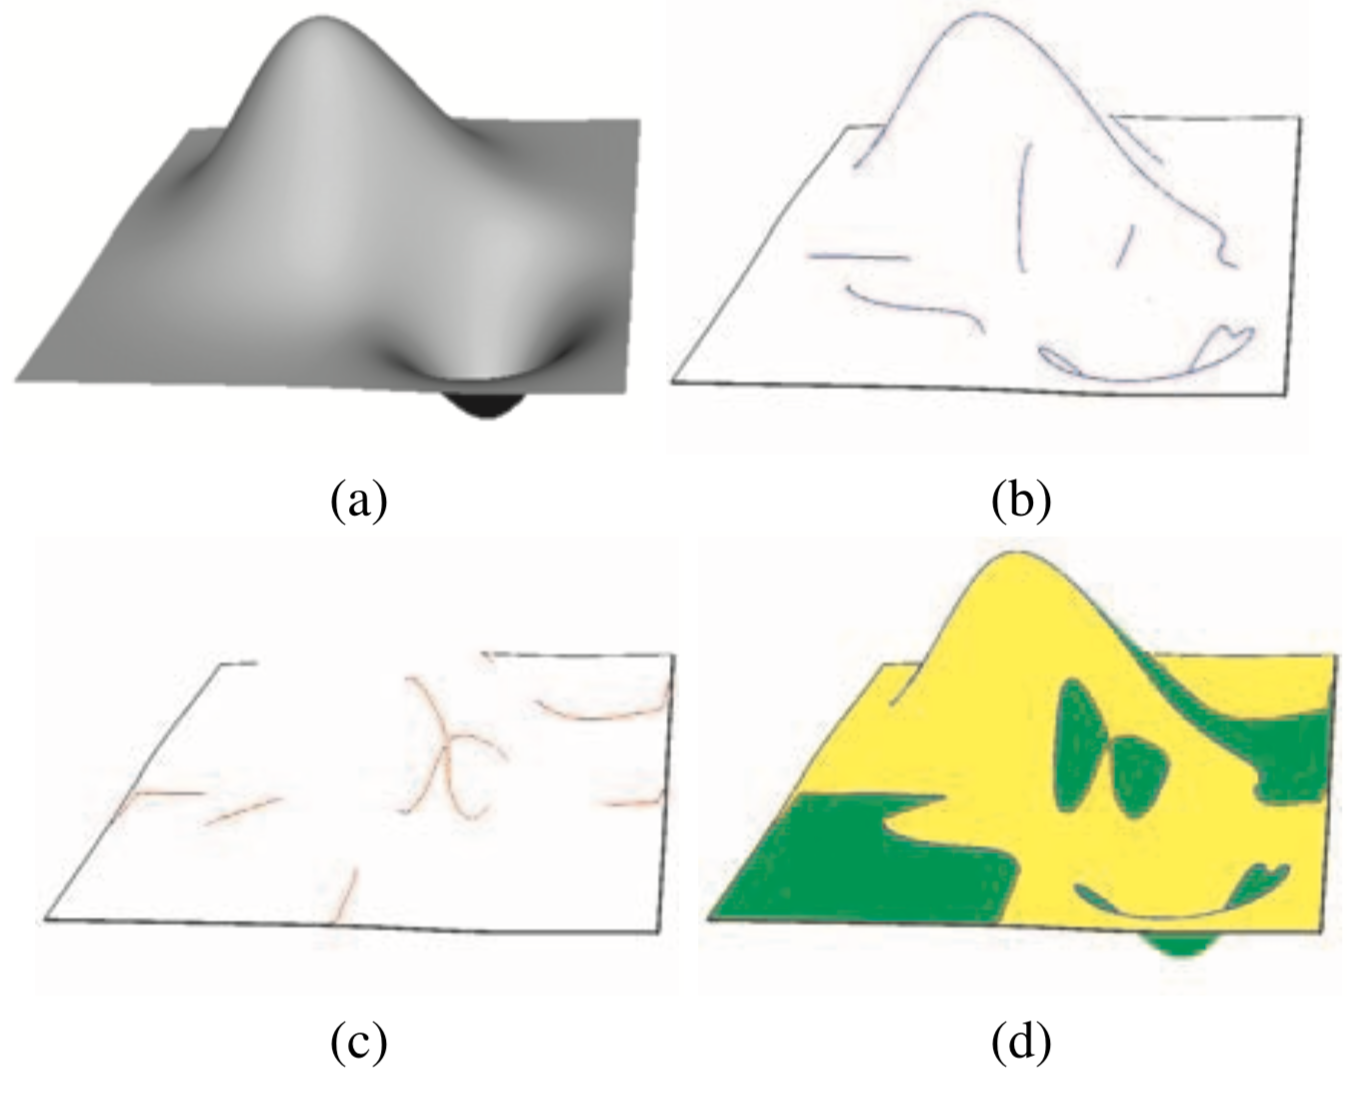
\includegraphics[width=0.7\linewidth]{abcd.png}
	\caption{(a): Die beleuchtete Oberfläche; (b): Die Maxima der zweiten partiellen Ableitung in Richtung des Gradienten. Diese werden für die PELs herausgefiltert; (c): Die Minima der zweiten partiellen Ableitung in Richtung des Gradienten; (d): Maxima und Minima ergeben geschlossene Bereiche, die sich dann in $D_{w}||\nabla f || < 0$ (gelb) und $D_{w}||\nabla f || < 0$ (grün) einteilen lassen. \cite{Xie2007}}
	\label{fig:abcd}
\end{figure}
\subsubsection{Beleuchtung}
Die Ausgangsfunktion der Berechnungen der Gradienten und somit der PEL stellt die Funktion $f$ dar, die das darzustellende Objekt beleuchtet.
Xie et al. wählen diesbezüglich das in der Computergrafik häufig verwendete Phong-Modell.
Dieses setzt sich zunächst aus drei verschiedenen Termen zusammen. Dem ambienten, dem diffusen und dem reflektierenden Term:
\begin{equation}
I = I_{amb} + I_{diff} + I_{spec}
\end{equation}
\\
Aufgrund der Tatsachen, dass der ambiente Term nicht zum Unterschied in der Beleuchtung (Kontrast) beiträgt und der reflektierende Term vom Sichtvektor abhängig ist, beziehungsweise an spiegelnden Stellen entstehende Feature Lines generell wenig über die Struktur des Objekts aussagen, vereinfachen Xie et al. das Modell zu:
\begin{equation}
I = I_{diff} = k_{d}I_{d}\mathbf{n}*\mathbf{l}
\end{equation}
\\\\
Zur Berechnung der Helligkeiten für jeden Punkt des Objekts genügen somit die Oberflächennormale $\mathbf{n}$ und der Lichtvektor $\mathbf{l}$. $k_{d}$ ist ein empirisch ermittelter Reflexionsfaktor für das Material des Objekts, $I_{d}$ ist die Lichtstärke.

\label{belfkt}
Da die Ergebnisse der PELs auch von der Positionierung der Lichter abhängen, schlagen Xie et al. eine von ihnen als am sinnvollsten getesteten Anordnung von Lichtern vor. Im Grunde bestehen diese aus einem Hauptlicht und optionalen Hilfslichtern.
\begin{description}
\item[Hauptlicht]\hfill \\
Das Hauptlicht ist ein gerichtetes Licht und beleuchtet das Objekt parallel zum Sichtvektor. Es ist zu beachten, dass dieses Licht mit der Kamera bewegt werden muss. Es entsteht eine Sicht-Abhängigkeit des Ergebnisses. \\
\item[Hilfslichter]\hfill \\
Die optionalen Spotlights sollen benutzerspezifizierte Bereiche besonders betonen. Diese sind lokal definiert und deshalb nicht von der Sicht abhängig.
\end{description}

Zur ergonomischen Positionierung der Hilfslichter wird weiterhin ein automatisches Verfahren vorgeschlagen, bei dem der Nutzer nur Bereiche des Objekts spezifizieren muss, die genauer oder weniger genau dargestellt werden sollen. Diese sind jeweils Teilmenge der gesamten Oberfläche:
\begin{equation}
\bar{S} \subseteq S
\label{eq:ssubsets}
\end{equation}
\\
Der Algorithmus sucht nun die Position $\mathbf{x}$ des Spotlights mit Richtungsvektor $\mathbf{d}$ und Zentrum der Teiloberfläche $\mathbf{c}$, sodass gilt:
\begin{equation}
\mathbf{d} = \frac{\mathbf{x} - \mathbf{c}}{||\mathbf{x} - \mathbf{c}||}
\end{equation}
und
\begin{equation}
max \int_{}\int_{\bar{S}} || \nabla f||^{2} dA
\end{equation}
für die Maximierung, oder
\begin{equation}
min \int_{}\int_{\bar{S}} || \nabla f||^{2} dA
\end{equation}
für die Minimierung der Beleuchtung der Teiloberfläche des Objekts. Die PELs für diese Bereiche werden dann mit den PELs des Hauptlichts ausgetauscht.
Es lassen sich so Feature Lines, und somit Details, hinzufügen, oder entfernen (Abbildung \ref{fig:rabbit}).
\\\\
Da die Beleuchtungsfunktion $f$ stetig ist, (siehe Abschnitt \ref{defpel}) und die PELs anhand der lokalen Maxima definiert werden,
sind an den Schnittpunkten der verschiedenen Bereichen keine Unstetigkeiten und damit ungewollte Feature Lines zu erwarten (Abbildung \ref{fig:rabbit}). Schnittpunkte entstehen dort, wo Punkte aneinander grenzen, die von verschiedenen Lichtern beleuchtet werden.
\\\\
Hervorzuheben ist, dass die Bereiche der Hilfslichter nicht von der Sicht abhängig sind und damit nur einmal berechnet werden müssen. Die Anzahl an Hilfslichtern beeinflusst also  nicht die Laufzeit einer Kamerabewegung.
\begin{figure}
	\centering
		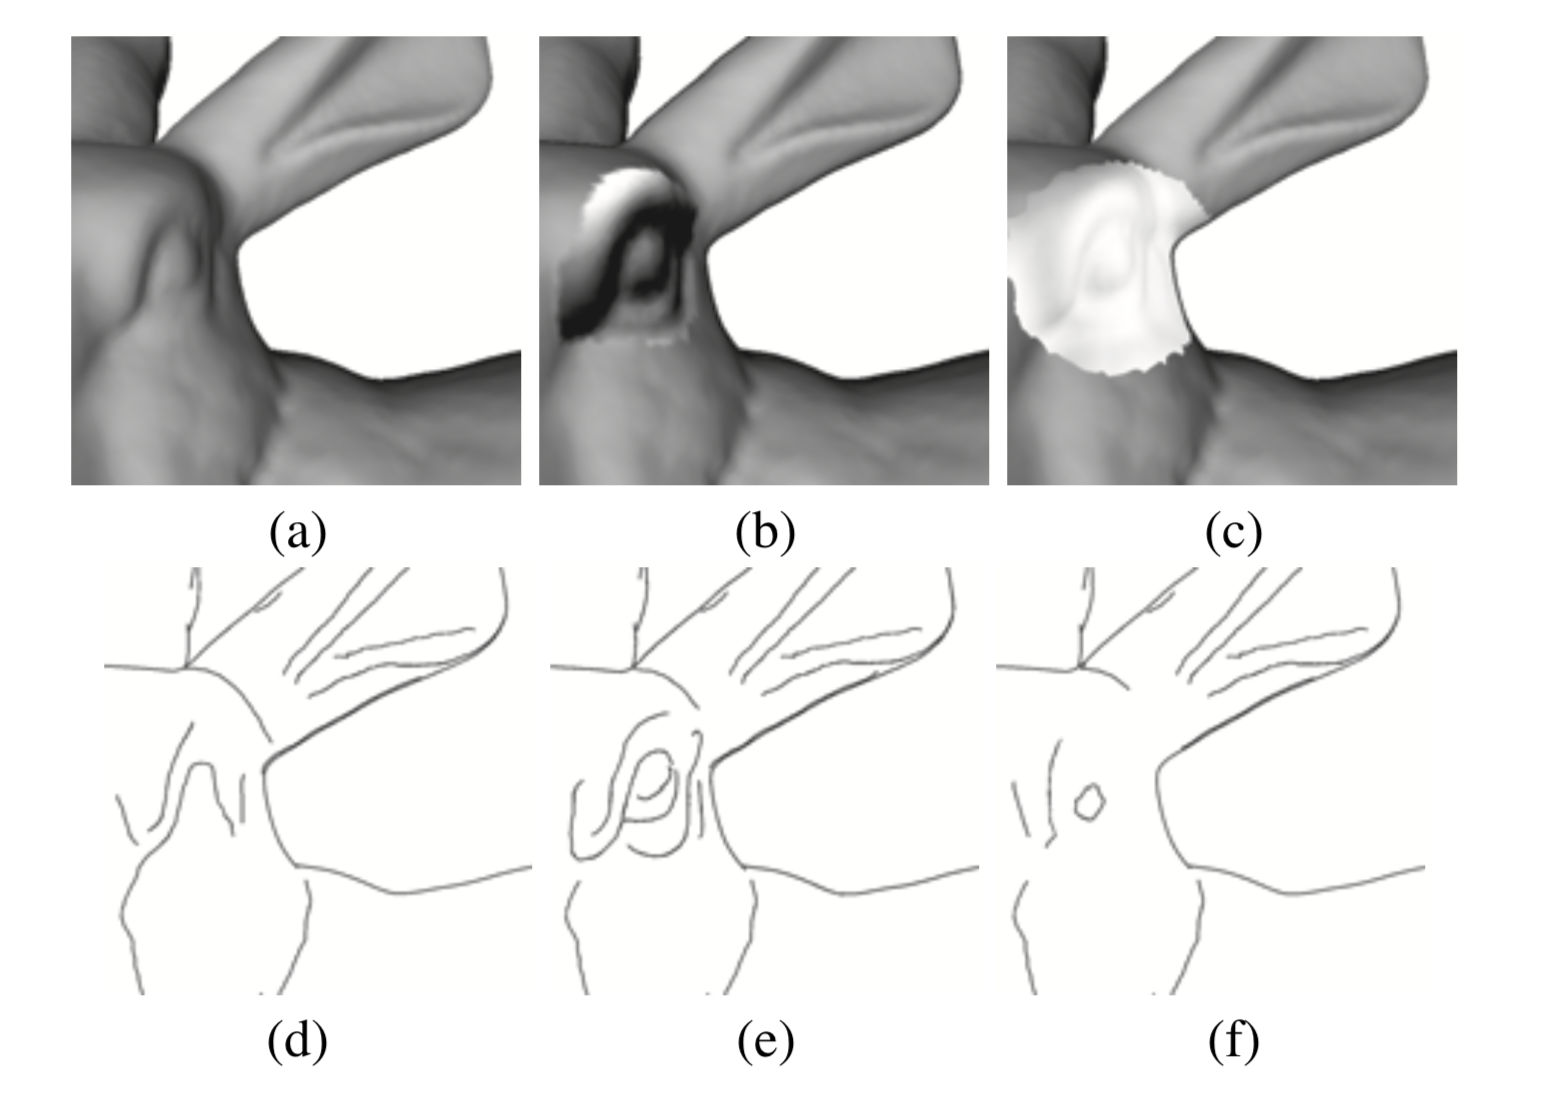
\includegraphics[width=0.7\linewidth]{rabbit.png}
	\caption{(a) und (d): Der nur durch das Hauptlicht beleuchtete Hase und zugehörige PELS. (b) und (c): Maximierung/Minimierung des Kontrasts der Beleuchtung des Bereiches um das Auge des Hasen mithilfe eines vor dem Auge positionierten Hilfslicht. (e) und (f): An den Grenzen der jeweiligen Bereiche sind in den zugehörigen PELs keine Unstetigkeiten erkennbar. \cite{Xie2007}}
	\label{fig:rabbit}
\end{figure}
\subsubsection{Implementationshinweise}
\label{pel-impl}
\textbf{Vorverarbeitung}\\
Da die Beleuchtungsfunktion $f$ stetig ist, kann mögliches unerwünschtes Rauschen nur durch eine zu detaillierte Geometrie entstehen. Xie et al. empfehlen deshalb, die Oberflächennormalen einmal zu Beginn des Algorithmus mit einem Bilateralfilter zu glätten. Das Vorgehen orientiert sich an Fleishman, Drori und Cohen-Or. Details lassen sich dem zugehörigen Paper \cite{Fleishman} entnehmen.\\\\
\textbf{Berechnen der Ableitungen}\\
Das Berechnen der (partiellen) Ableitungen bildet einen Großteil der zum Finden der PELs benötigten Schritte (vergleiche Abschnitt \ref{defpel}). Da die Oberfläche allerdings üblicherweise nicht als Funktion $S : D \subset R^{2} \longrightarrow R^{3}$, sondern als Menge einzelner Punkte gegeben ist, können Ableitungen nicht implizit berechnet werden. Xie et al. bedienen sich deshalb eines Tricks:
Die Berechnung der Ableitung eines Punktes erfolgt durch Mitteln der Ableitungen der anliegenden Dreiecke. Diese berechnen sich durch:
\begin{equation}
\resizebox{.85\hsize}{!}{$\nabla g = \left(\begin{array}{c}\frac{\partial g}{\partial x} \\ \frac{\partial g}{\partial y}\end{array}\right) = \frac{1}{d_{T}} \left(\begin{array}{rrr}y_{2}-y_{3} & y_{3}-y_{1} & y_{1}-y_{2} \\ x_{3}-x_{2} & x_{1}-y_{3} & x_{2}-x_{1}\end{array}\right) \left(\begin{array}{c}g_{1} \\ g_{2} \\ g_{3}\end{array}\right)$}
\label{eq:derivativepel}
\end{equation}
\\
$g_{1}$, $g_{2}$ und $g_{3}$ sind die Helligkeitswerte der drei Punkte des Dreiecks. Die x- und y-Werte sind die Koordinaten der Punkte im Koordinatensystem des Dreiecks und $d_{T}$ der doppelte Flächeninhalt des Dreiecks. Diese Ableitungen müssen in das jeweilige Punktkoordinatensystem überführt werden. Dies geschieht durch Multiplikation mit den Tangentenvektoren des Punktes:
\begin{equation}
\nabla g(u_{i},v_{i}) = \left(\begin{array}{c}\mathbf{u_{i}} \cdot \nabla g(x,y) \\ \mathbf{v_{i}} \cdot \nabla g(x,y)\end{array}\right)
\label{guivui}
\end{equation}
\\
Sind alle Ableitungen der anliegenden Dreiecke des Punktes berechnet und in das korrekte Koordinatensystem überführt, werden diese mittels Voronoi-Flächengewicht $w_{i}$ gemittelt und aufaddiert. Das bedeutet, dass nur der Anteil des jeweiligen Dreiecks verwendet wird, der auch am nähesten an diesem Punkt liegt. Weitere Informationen zum Ermitteln der Gewichtung $w_{i}$ ist der Quelle \cite{Voronoi} zu entnehmen.
Die Ableitung eines Punktes berechnet sich demnach abschließend mittels der Formel:
 \begin{equation}
\nabla g(u,v) = \sum_{i} w_{i} \nabla g(u_{i},v_{i})
\label{guvl}
\end{equation}
\\
\textbf{Zeichnen der PELs}\\
Um die Photic Extremum Lines zu zeichnen, muss zunächst die genaue Positionierung der Nullstellen gefunden werden, da diese zumeist nicht direkt auf den Punkten des Objekts liegen. Eine Nullstelle zwischen zwei Punkten liegt genau dann vor, wenn die berechneten partiellen Ableitungen der Gradienten verschiedene Vorzeichen besitzen. Liegt eine Nullstelle vor, muss deren genauer Ort durch lineare Interpolation bestimmt werden. Dafür legen Xie et al. zunächst fest, dass $h(\mathbf{v}) = D_{w}|| \nabla f(\mathbf{v})||$. Die Interpolation ist dann gegeben durch:
\begin{equation}
\mathbf{p} = \frac{|h(\mathbf{v}_{2})|\mathbf{v}_{1}+|h(\mathbf{v}_{1})|\mathbf{v}_{2}}{|h(\mathbf{v}_{2})|+|h(\mathbf{v}_{1})|}
\end{equation}
\\
Werden zwei Nullstellen auf Kanten eines Dreiecks gefunden, kann zwischen diesen beiden Punkten eine Linie gezeichnet werden.
\\\\
\textbf{Schwellwert}\\
Xie et al. empfehlen, einen zusätzlichen Schwellwert einzubinden, der diejenigen PELs entfernt, die generell unnötige kleine Details beschreiben. Es wird dabei eine Größe berücksichtigt, die sich auch als die Stärke einer Linie betrachten lässt. Hierfür bedient sich die Gruppe einer Technik von Ohtake et al. \cite{Ohtake} und integriert $|| \nabla f ||$über die einzelnen Linien.
\begin{equation}
\resizebox{.88\hsize}{!}{$\int{} || \nabla f ||ds \approx \sum \frac{ \nabla f(\mathbf{p}_{i})|| + || \nabla f(\mathbf{p}_{i+1})||}{2}||\mathbf{p}_{i} - \mathbf{p}_{i+1}||$}
\end{equation}
Liegt der berechnete Wert unter einem vom Nutzer gesetzten Schwellwert, wird die Linie gelöscht.
\section{Ergebnisse/Anwendungen/Diskussion}
In diesem Abschnitt sollen die Ergebnisse der zugrundeliegenden Paper der Arbeit kurz vorgestellt werden. Dazu werden Demarcating Curves und Photic Extremum Lines zunächst kurz miteinander, danach mit anderen gängigen Feature-Line-Methoden verglichen. Anschließend wird auf Anwendungsgebiete und Performance eingegangen. 
\subsection{Vergleich}
\subsubsection{Demarcating Curves und Photic Extremum Lines}
Vergleicht man die hier vorgestellten Methoden, stellt man fest, dass viele Konzepte in beiden Algortihmen angewendet werden. Bei den Demarcating Curves wird der Gradient der Krümmung genutzt, um interessante Punkte zu markieren. Bei den PELs werden die Punkte anhand des Gradienten der Beleuchtung ermittelt. In beiden Fällen wird also eine starke Veränderung einer Eigenschaft zum Marker für wichtig erscheinende Regionen. Betrachtet man die Ergebnisse der beiden Algorithmen (Abschnitt \ref{ergebnis}), lassen sich auch hier Ähnlichkeiten erkennen. Diese sind möglicherweise dadurch zu erklären, dass die markanten Punkte der eigentlichen Geometrie einer Oberfläche eben die Punkte sind, die Veränderungen der Helligkeit bei der Beleuchtung hervorrufen. 

Die Demarcating Curves schaffen es, auch sehr feine Strukturen blick-unabhängig hervorzuheben. PELs sind dagegen immer abhängig von der Position der Lichter. Somit können Abweichungen auf der Oberfläche parallel zum Sichtvektor aufgrund der frontalen Beleuchtung verschwinden. 
\subsubsection{Vergleich mit anderen Methoden}
Die Autoren vergleichen in ihren Arbeiten die Demarcating Curves \cite{Demarcating} und Photic Extremum Lines \cite{Xie2007} mit einigen anderen verbreiteten Methoden. Beispielhaft wird hier auf die Vergleiche zu Suggestive Contours, sowie zu Ridges \& Valleys eingegangen. Für eine umfangreichere Ausführung und den Vergleich mit weiteren Methoden wird auf die Quellen verwiesen. 
\begin{figure*}
	\centering
	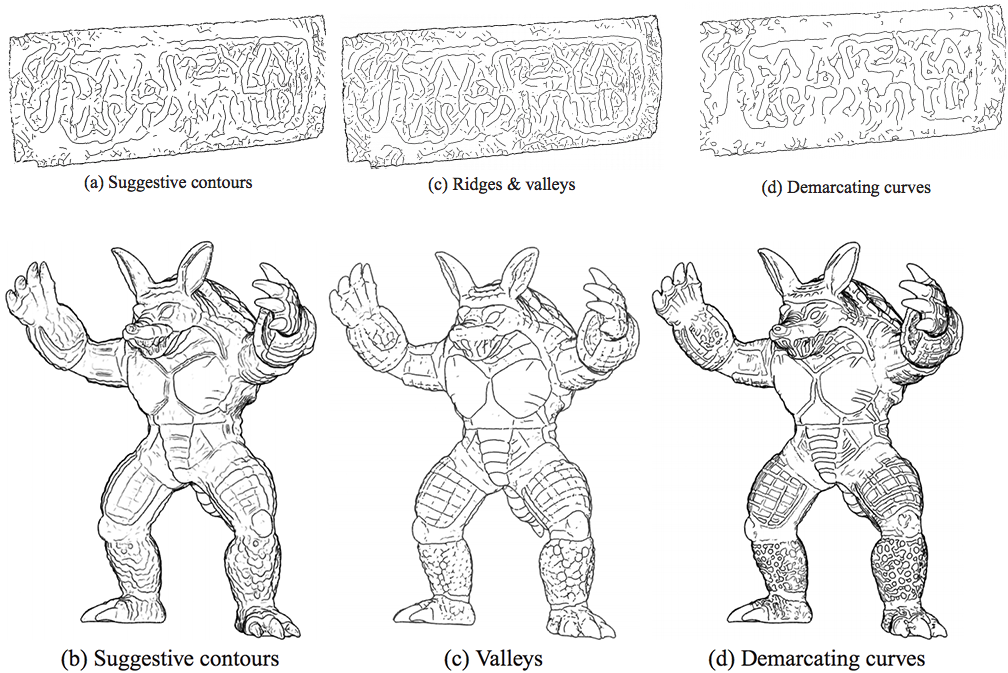
\includegraphics[width=0.8\linewidth]{demvgl.png}
	\caption{Scan eines Relikts. Beleuchtet mit exaggerated shading. Es zeigt die Kombination von Demarcating Curves und Beleuchtungsmethoden. \cite{Demarcating}}
	\label{im:demvgl}
\end{figure*}

\textbf{Vergleich: Suggestive Contours}\\
Da sowohl die Suggestive Contours, als auch die Demarcating Curves auf hyperbolen Regionen (also Regionen mit negativer Gauskrümmung) der Oberfläche liegen, lassen sich bei der Betrachtung viele Übereinstimmung bei den hervorgehobenen Strukturen erkennen. Genauer sind die Kurvenpunkte der Demarcating Curve eine Teilmenge der Vereinigung aller Suggestive Contours Punkte, aus allen möglichen Blickrichtungen betrachtet \cite{Demarcating}(siehe Abbildung: \ref{im:demvgl}).  

Die Photic Extremum Lines zeigen ihren Unterschied gegenüber den Suggestive Contours vor allem bei der Darstellung von Objekten, in denen sowohl konkave, als auch konvexe Oberflächen zu finden sind. Während bei Suggestive Contours ein Schwellwert gewählt werden muss, der meistens dafür sorgt, dass entweder konkave, oder konvexe Flächen detailliert dargestellt werden, so ist es mit den PELs möglich, beide Bereiche gleichzeitig darzustellen \cite{Xie2007}. Ersichtlich wird dies in Abbildung \ref{vglpel2}.

\textbf{Vergleich: Ridges \& Valleys}\\
Gegeben der Idee von Demarcating Curves (siehe \ref{defdem}) liegt die Vermutung Nahe, dass die Kurven zwischen den ''Hügeln und Tälern'' (Ridges \& Valleys) auf der Oberfläche verlaufen. Mathematisch lässt sich diesen Idee zwar modellieren \cite{Demarcating}, in der Praxis liegen die Demarcating Curves allerdings nicht zwischen den Kurven der Ridges \& Valleys. In Abbildung \ref{im:demvgl} wird außerdem deutlich, dass besonders abgeschlossene Strukturen (z.B. auf den Beinen der Figur) durch die Demarcating Curves deutlich besser hervorgehoben werden, als durch die Valley.

Die Ergebnisse der Photic Extremum Lines weichen von denen der Ridges \& Valleys besonders bei der Darstellung weicher Strukturen ab.
Weil Ridges \& Valleys mit der Stärke der Krümmung der Geometrie und nicht mit dem beleuchteten Objekt arbeiten, werden weiche Übergänge, die sich erst mittels Beleuchtung des Objekts bemerkbar machen, vernachlässigt (siehe Abbildung \ref{vglpel2}). 
\begin{figure}
	\centering
		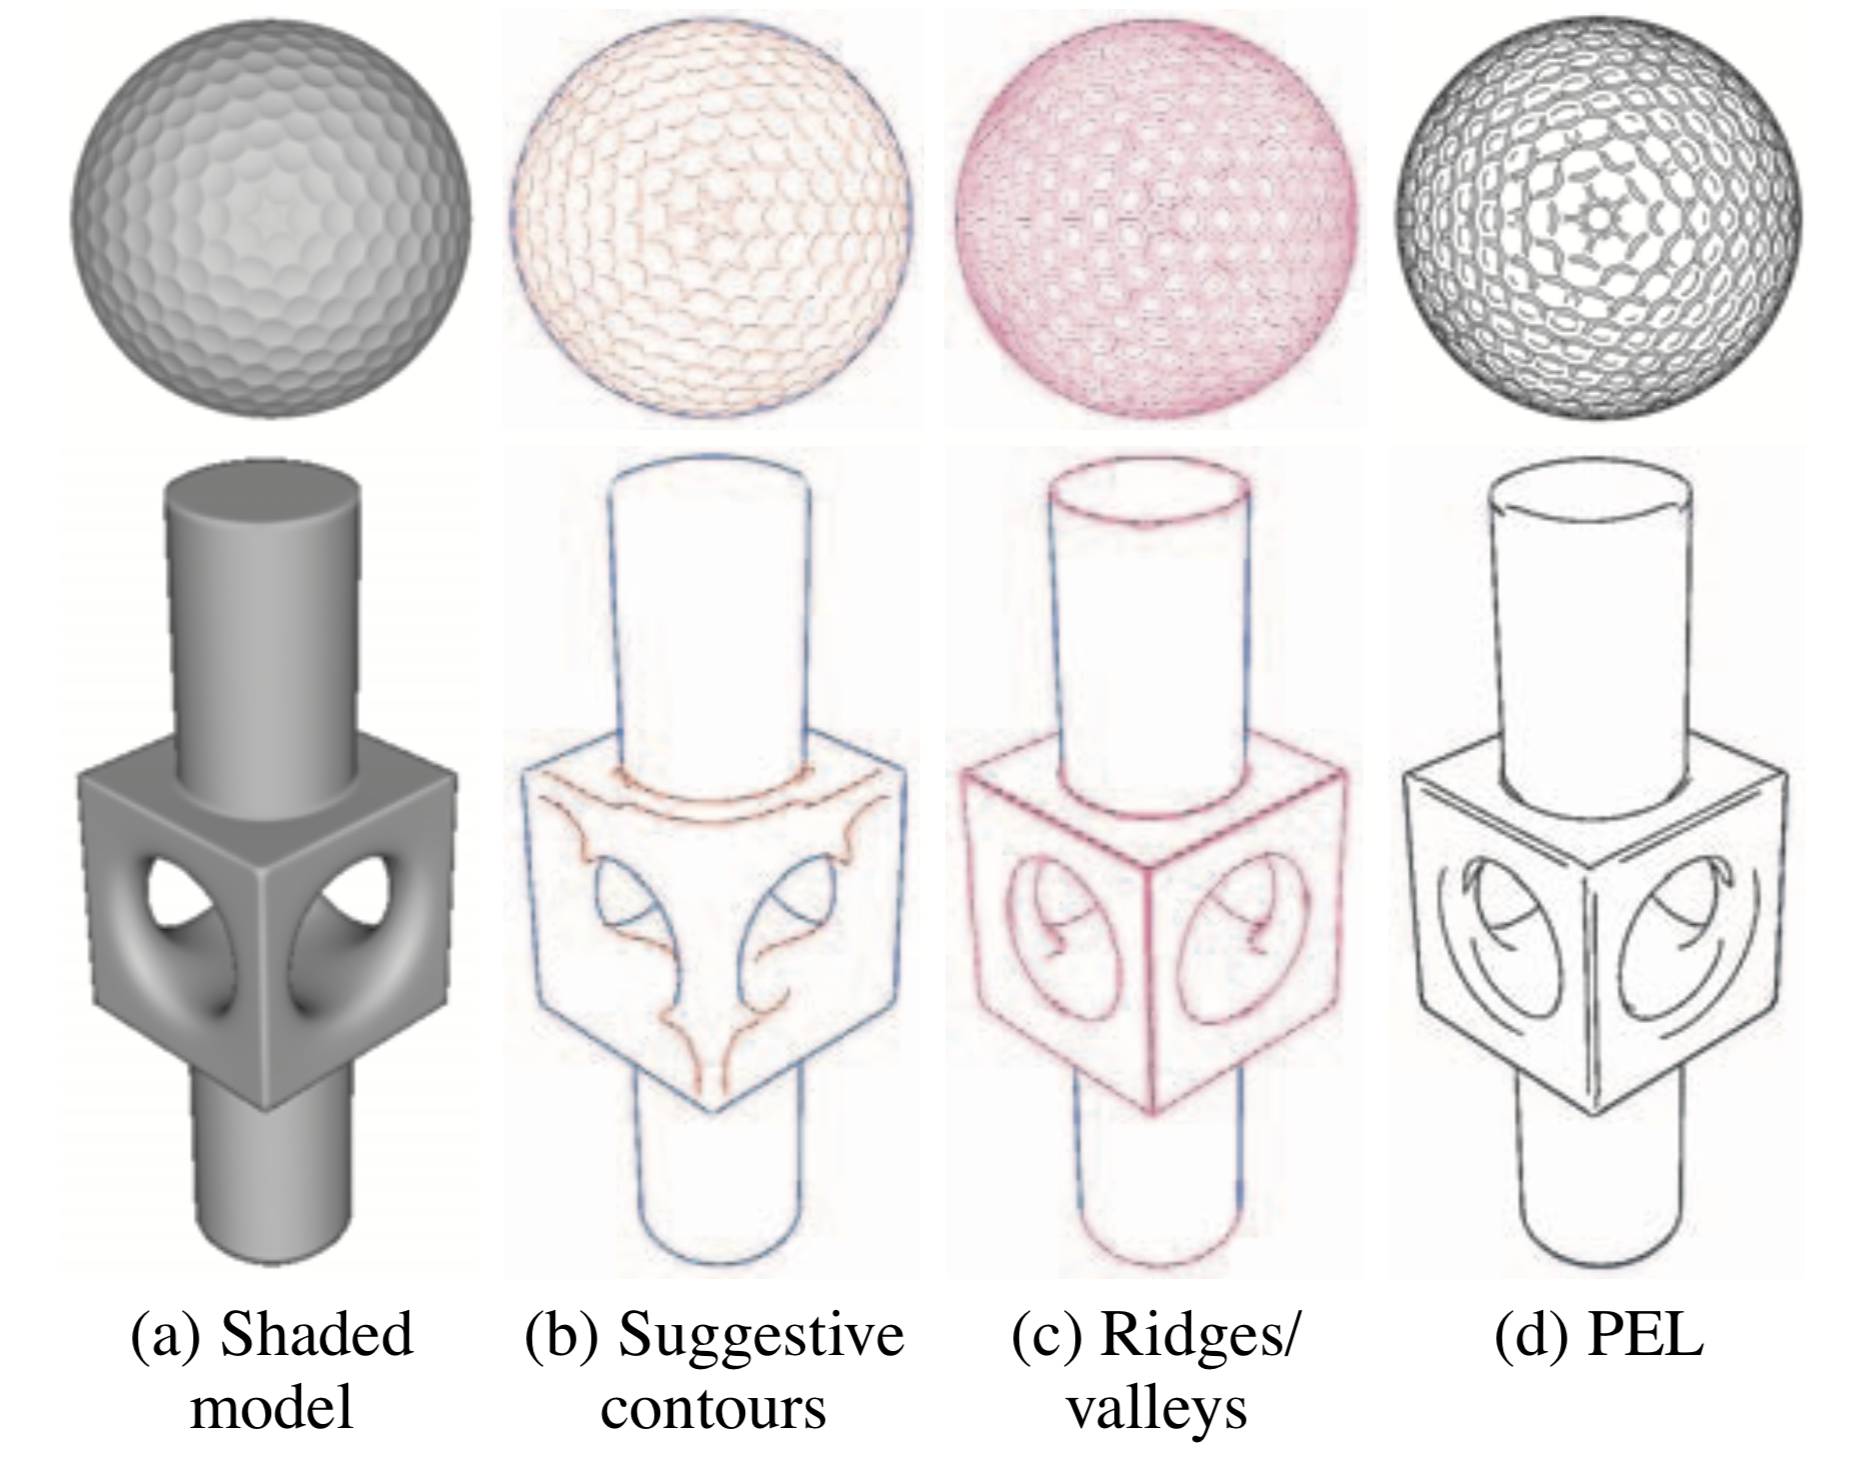
\includegraphics[width=0.9\linewidth]{vglpel2.png}
	\caption{Die Darstellung eines künstlich erstellten Objekts mittels PEL im Vergleich zu anderen Feature Line Methoden \cite{Xie2007}.}
	\label{vglpel2}
\end{figure}
\subsection{Performance}
Bei der Bestimmung von Demarcating Curves findet die gesamte Berechnung offline, also vor der Interaktion mit den Nutzern statt. Damit sind sie genauso schnell zu Berechnen wie die genannten Suggestive Contours und Ridges \& Valleys. Als einzige interaktive Komponente nennen Kolomenkin et al. \cite{Demarcating} einen Stärkeparameter, der als Schwellwert für die Vorberechneten Werte der Krümmungsableitung in Gradientenrichtung ($C_{ijk}g_p^ig_p^jg_p^k$) dient. Durch diesen Schwellwert lassen sich schwächere Kandidaten für die Kurvenpunkte eliminieren. Auf einem Testsystem (2.66 GHz Intel Core Duo) konnten die Autoren ein Mesh aus 50.000 Polygonen in 0.15 Sekunden bearbeiten. Für ein Mesh aus 500.000 Polygonen benötigte der Algorithmus 1.1 Sekunden. 

Der Performance-Test der Photic Extremum Lines wurde von Xie et al. \cite{Xie2007} auf einem Desktop PC mit 3.2 GHz Xeon-Prozessor und 3GB Arbeitsspeicher durchgeführt. Die getesteten Modelle sind die im Paper verwendeten. Zwar ist das Verfahren auf komplizierten Objekten nicht Echtzeit-fähig, die Betrachtung sollte aber mit aktueller Technik zumindest bei simplen Modellen zufriedenstellend flüssig laufen.
Wichtig ist zu erwähnen, dass sich diese Zeiten nur auf eine Betrachtung mit Kamerabewegung auswirken. Wird das Modell nur aus einer bestimmten Richtung betrachtet, kann der Zeitaufwand zur einmaligen Berechnung vernachlässigt werden. 
\begin{table}[htb]

\begin{tabular}{|l|ll|}
\hline
Modell & $\#\bigtriangleup$ & Sekunden/Frame\\
\hline
Synth. Oberfläche. & 44K & 0.170 \\
Max-Planck & 98K & 0.350 \\
Hase & 144K & 0.515 \\
Kopf & 320K & 1.684 \\

\hline
\end{tabular}
\caption{Performance der Photic Extremum Lines. Die zugehörigen Modelle sind in den Abbildungen \ref{vglpel2}, \ref{anwpel}, \ref{fig:rabbit} und \ref{ausblpel} zu sehen.  \cite{Xie2007}} 
\label{tab:TableExample}
\end{table}

\subsection{Ergebnisse und Anwendung}
\label{ergebnis}
\begin{figure*}
	\centering
		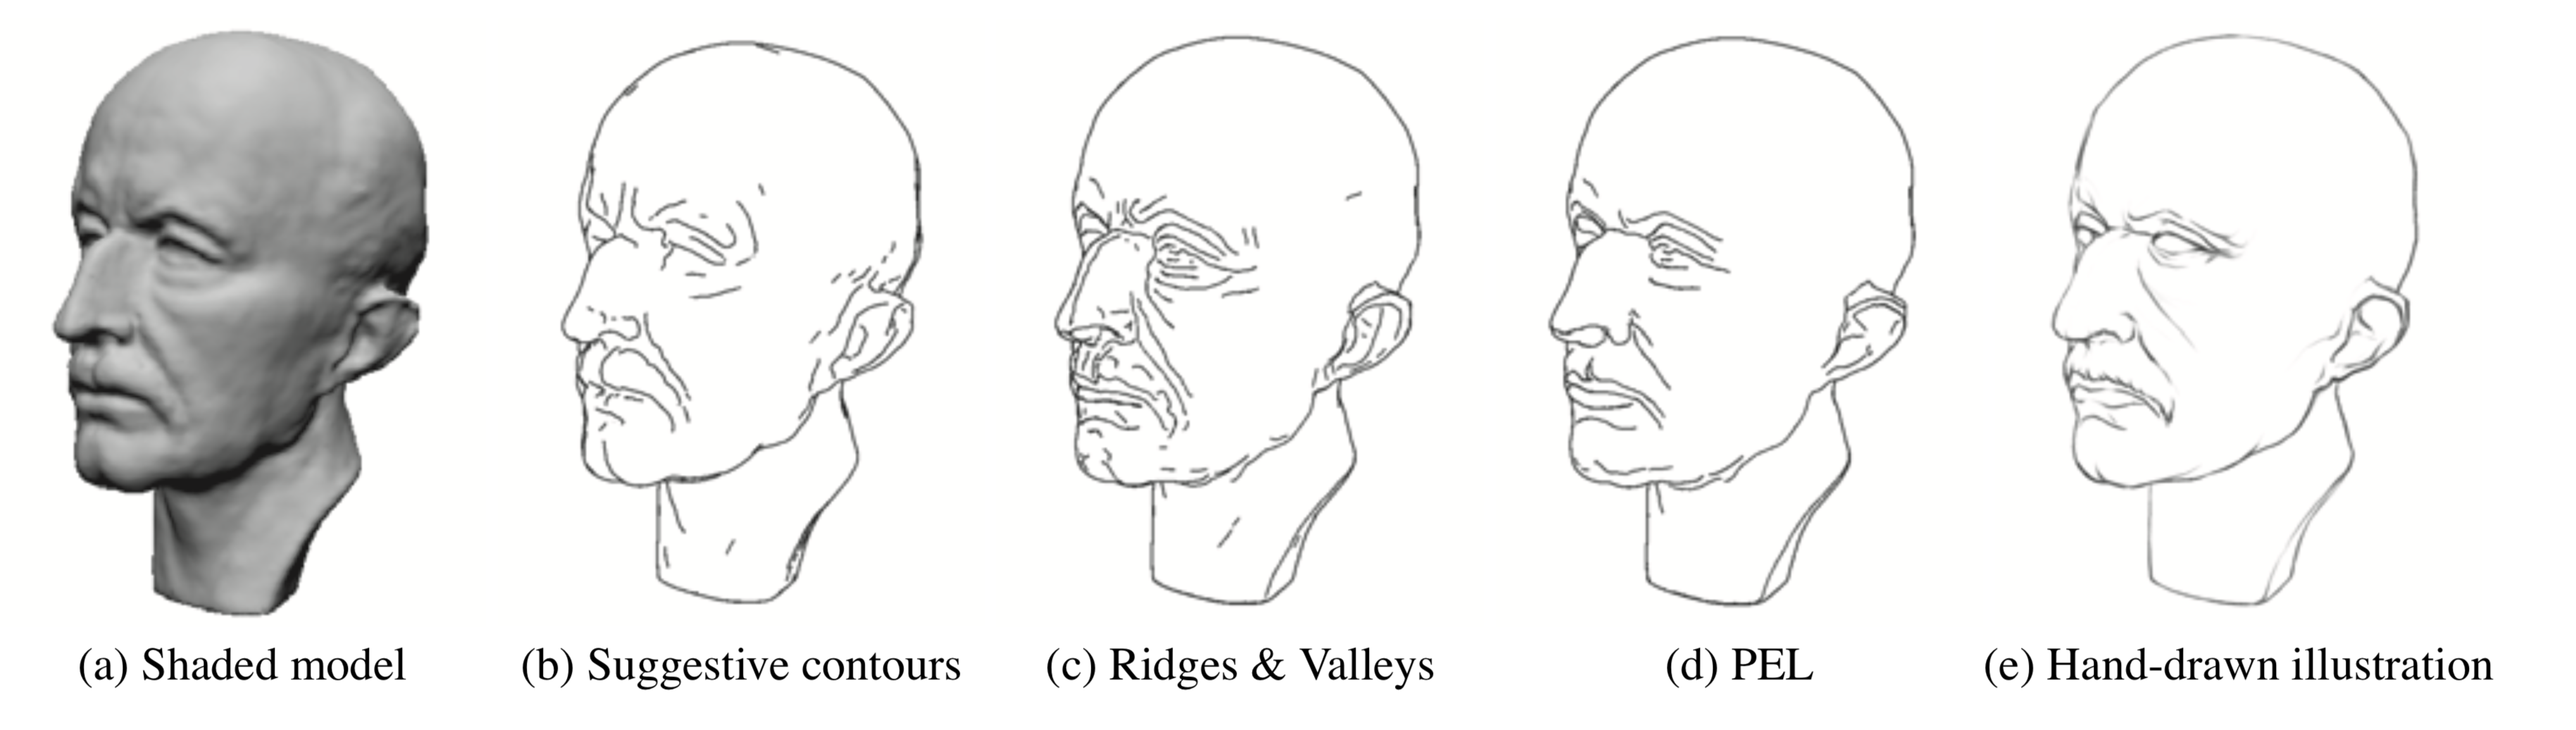
\includegraphics[width=0.9\linewidth]{anwpel.png}
	\caption{Die Darstellung eines Kopfes mittels Photic Extremum Lines und anderer Feature Line Methoden im Vergleich zu einer von einem Künstler angefertigten Zeichnung. Es wird die große Übereinstimmung von den Linien des Zeichners und den Linien der PELs deutlich. \cite{Xie2007}}
	\label{anwpel}
\end{figure*}
Mit den Demarcating Curves stellen Kolomenkin et al. eine neue Art von Kurven vor, die markante Strukturen auf Oberflächen hervorhebt. Im Vergleich mit anderen etablierten Feature Line Methoden bieten die Demarcating Curves einen Mehrwert und erfassen auch Strukturen, die von den bekannten Feature Line Methoden nicht erfasst werden können. Vor dem Hintergrund der Anwendung in einem archäologischen Kontext sind die neuen Kurven scheinbar gut geeignet. In einer Befragung von Fachleuten stießen die Demarcating Curves bei der illustrativen Darstellung von Relikten auf größtenteils positives Feedback. Im direkten Vergleich mit Darstellungen aus anderen Methoden bevorzugten die Fachleute meist Demarcating Curves. Insbesondere in Kombination mit einem beleuchteten (shaded) Modell (Abbildung: \ref{im:shadedDem})erzielen die Kurven optisch ansprechende Ergebnisse. \cite{Demarcating}

Die Photic Extremum Lines charakterisieren die signifikanten Variationen der Beleuchtung auf 3D-Oberflächen. Dabei stehen dem Nutzer durch die Anzahl der Lichtquellen, die Lichtposition(en), und den Schwellwert eine hohe Auswahl an Anpassungsmöglichkeiten zur Verfügung. Da die Ergebnisse sehr stark an ein von Künstlern gezeichnetes Bild erinnern (siehe Abbildung \ref{ausblpel}) und damit unserer eigenen Wahrnehmung des Objekts sehr nahe kommen, können Photic Extremum Lines insbesondere für Anwendungen interessant sein, die sich auf die verständliche und illustrative Darstellung von Objekten konzentrieren. Auch eine von Xie et al \cite{Xie2007} durchgeführte Befragung unter Künstlern besagt, dass 9 von 10 Künstlern die Ergebnisse der PELs den der anderen vorgelegten Verfahren (Suggestive Contours, Ridges \& Valleys) vorziehen würden. 
\section{Zusammenfassung/Schlussfolgerung/Ausblick}

\begin{figure}
	\centering
	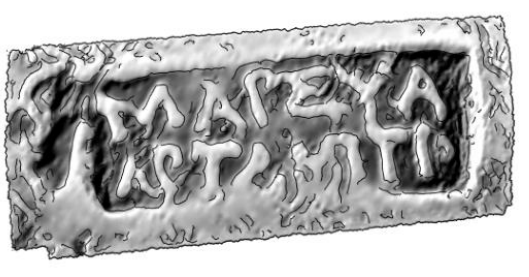
\includegraphics[width=0.9\linewidth]{shadedDem.png}
	\caption{Scan eines Relikts. Beleuchtet mit exaggerated shading. Es zeigt die Kombination von Demarcating Curves und Beleuchtungsmethoden. \cite{Demarcating}}
	\label{im:shadedDem}
\end{figure}

\begin{figure}
	\centering
		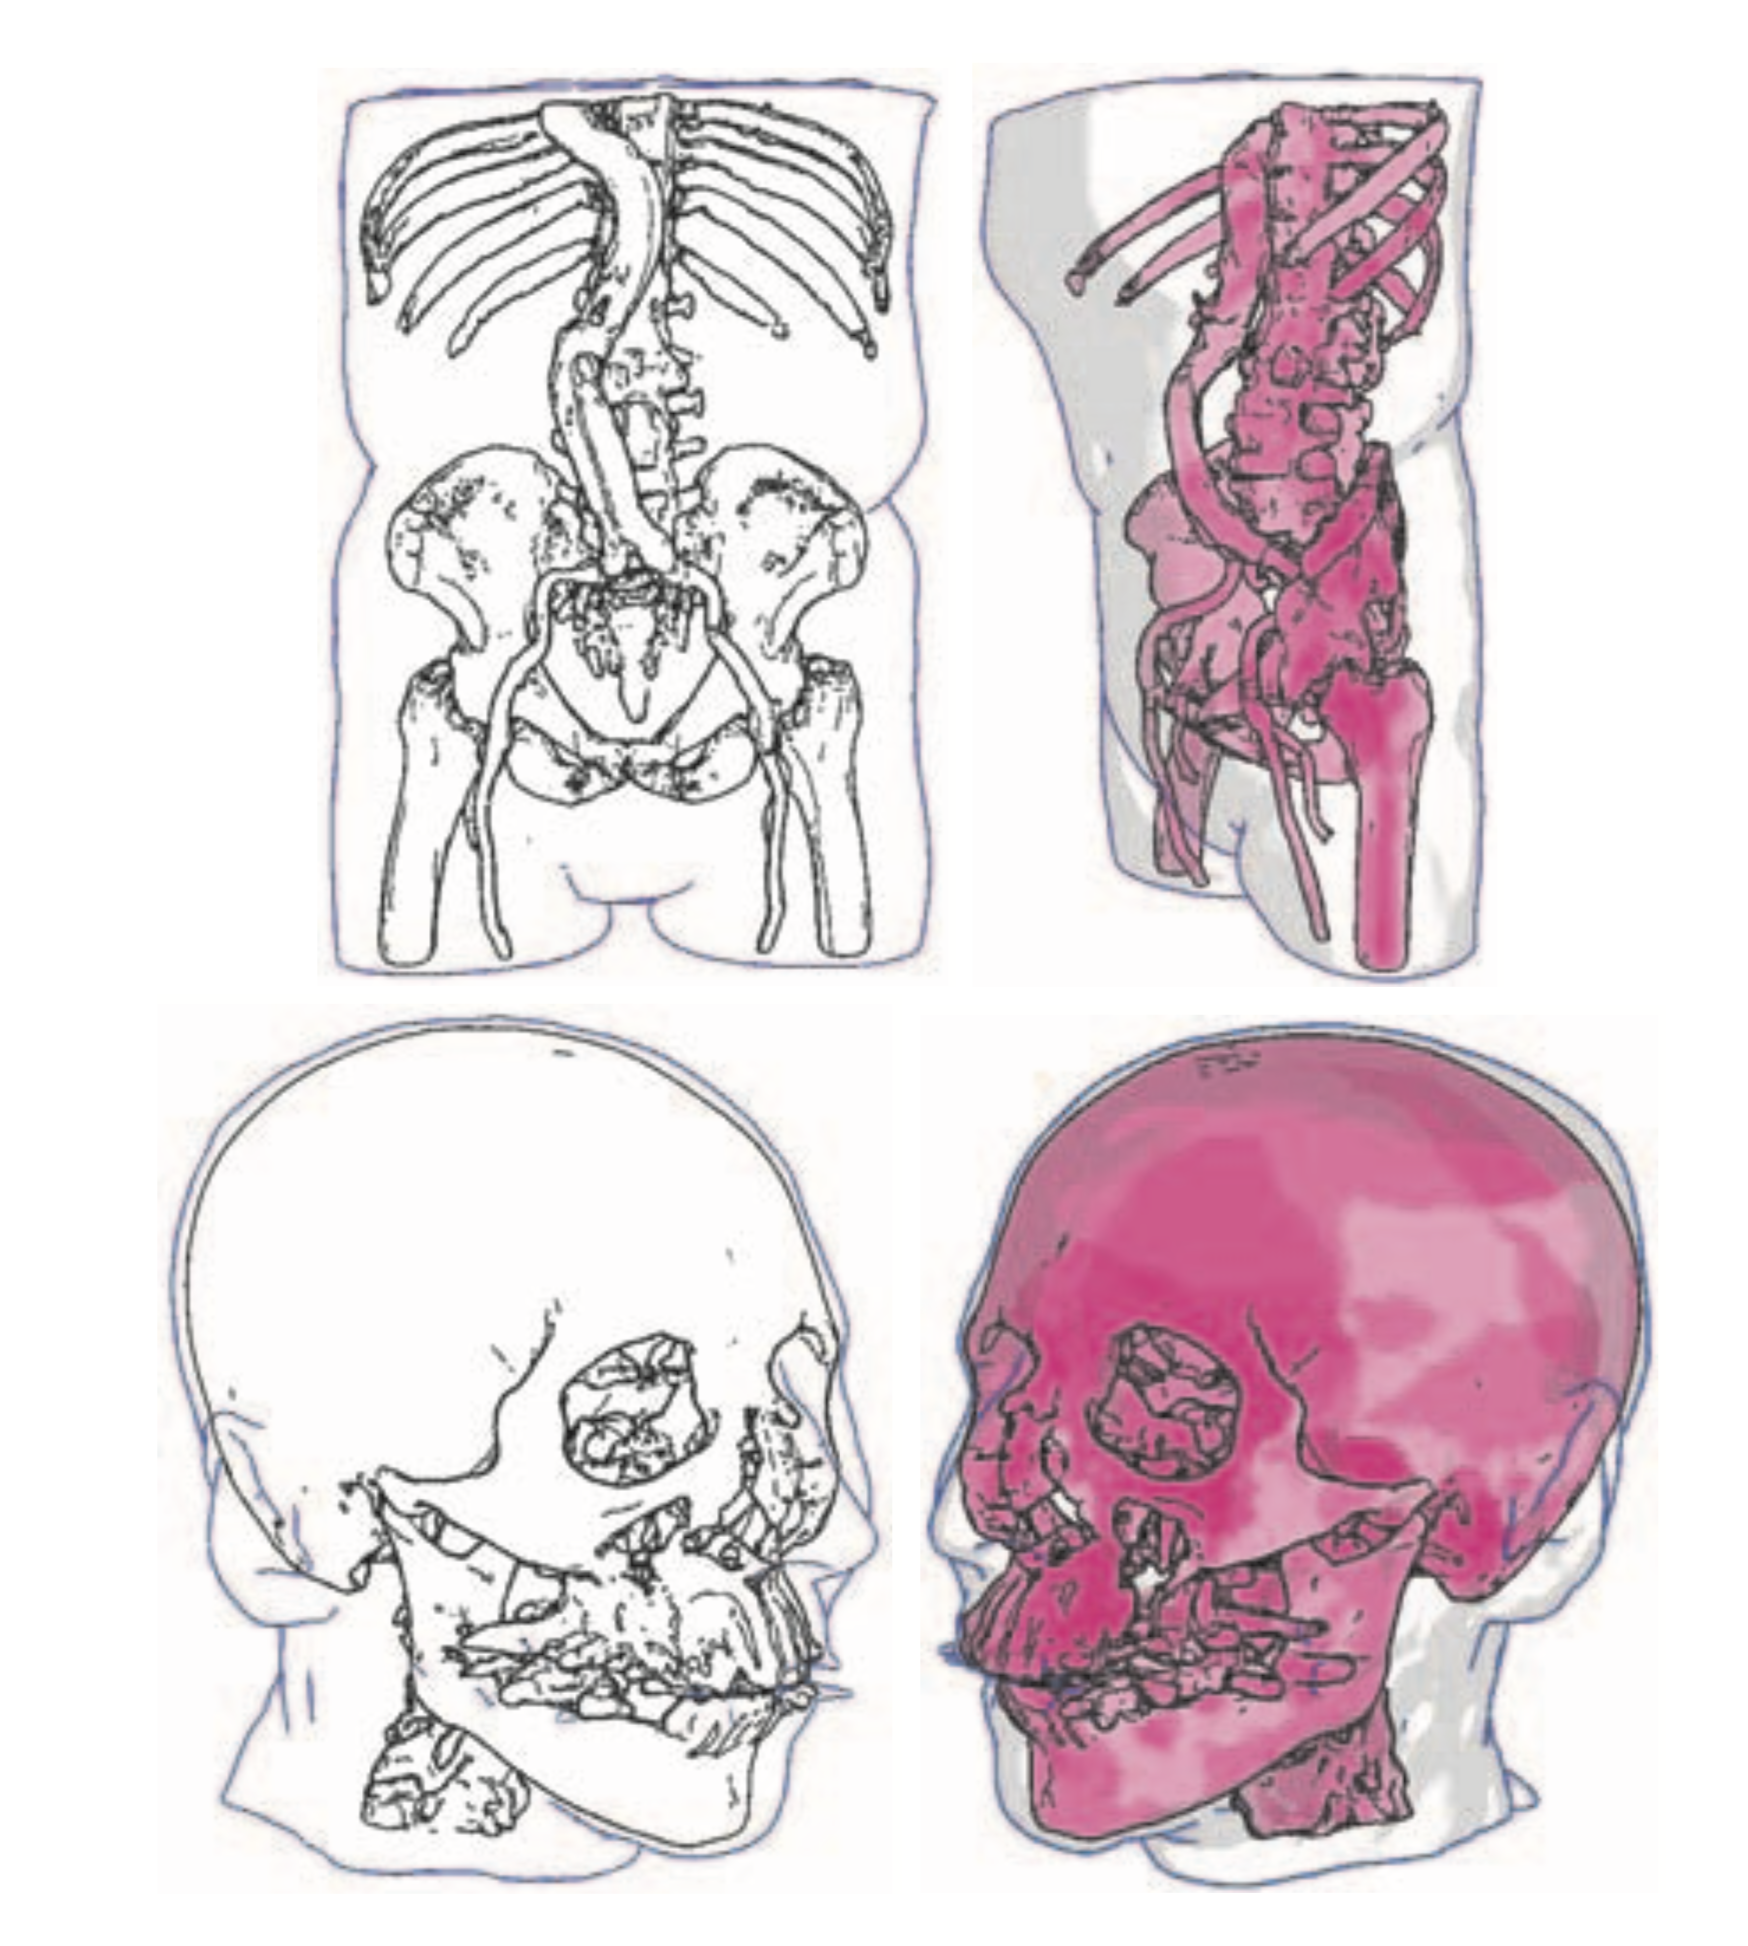
\includegraphics[width=0.9\linewidth]{ausblpel.png}
	\caption{Die Darstellung eines Volumen-Scans mittels Photic Extremum Lines. Die äußeren Grenzen des Körpers sind durch einfachen Konturen dargestellt. Die Knochenstruktur (rechts eingefärbt) wurde zuvor als Isofläche aus dem Dichtefeld des Scans extrahiert. Als Ausblick ihrer Arbeit erwähnen Xie et al. eine direkte Darstellung ohne vorherige Extraktion. \cite{Xie2007}}
	\label{ausblpel}
\end{figure}
In dieser Arbeit wurden mit den Demarcating Curves und den Photic Extremum Lines zwei Methoden zum Finden von Feature Lines auf polygonalen Oberflächen vorgestellt. Die beiden Methoden ergänzen die bisher bekannten Algorithmen und liefern vergleichbare Ergebnisse. Demarcating Curves arbeiten dabei auf der eigentlichen Geometrie und betrachten Krümmungseigenschaften, die Photic Extremum Lines suchen nach maximalen Unterschieden in der Beleuchtung eines Objekts. 

Es lässt sich abschließend sagen, dass nicht jede Methode für jedes Anwendungsgebiet gleichermaßen gut geeignet ist. In bestimmten Aufgabenfeldern sind von Menschen gezeichnete Konturen und Linien immer noch der qualitative Standard. Die beiden vorgestellten Methoden lieferten allerdings gute Ergebnisse auf ihren Gebieten und positives Feedback von Fachexperten (Archäologen und Künstler).

Für die weitere Verwendung der Demarcating Curves schlagen Kolomenkin et al. \cite{Demarcating} vor, die aus den Kurven gewonnenen Informationen weiter zu verwenden.Sie nennen hier die digitale Archivierung und den bildbasierten Vergleich von Fundstücken.  
Die Gruppe um Xie nennt als Ausblick die weitere Verbesserung der Performance durch Optimierung der Implementation und das direkte Zeichnen von PELs aus Volumendaten ohne vorherige Extraktion von Isoflächen (siehe Abbildung \ref{ausblpel}). 

%-------- *.bib file with references and style file
\bibliographystyle{literaturStyle}
\bibliography{literatur}
\end{document}
#